\begin{savequote}[75mm]
This is a really enlightening quote. 
\qauthor{Tomo Lazovich}
\end{savequote}

\chapter{Combined limits from boosted and resolved searches}
\label{chap:4bcomb}

\section{Introduction}

In order to cover the full mass range of possible resonances decaying to di-Higgs final states, two distinct tailored selections were produced. The resolved selection is more sensitive in the mass range of $400 < m_{X} < 1100 \GeV$ while the boosted selection is more sensitive to masses in the range $1100 < m_{X} < 3000 \GeV$. Chapter 7 presents the details of the boosted selection and results. In setting limits on spin-2 Randall-Sundrum graviton (RSG) and narrow width heavy scalar ($H$) models, the results of the boosted selection are combined with the results of the resolved selection to cover the full mass range.

This chapter presents limits on signal models resulting from the $\FourBfull$ search in both the resolved and boosted selections. It first presents a brief overview of the resolved results that go into the limit setting. Then, an overview of the statistical methods used for the search and limit setting is given. Finally, limits on the RSG and heavy scaler models are presented. 

\section{Resolved results}

The details of the resolved selection will not be presented here and can be found in reference~\cite{4bconf}. In basic terms, the selection searches for four $R = 0.4$ b-tagged calorimeter jets (where each pair of jets is one Higgs candidate). This is distinct from the boosted methodology which searches for merged decay products. The backgrounds to the resolved selection are the same as those presented in Chapter 7 for the boosted analysis. 

Table~\ref{tab:ResolvedResults} shows the results for data yields and expected background in the resolved signal region. Figure~\ref{fig:ResolvedResults} shows the $M_{2J}$ distribution in the resolved signal region. The total number of events is consistent with the prediction and no significant excess is seen.

\begin{table}[!ht]
\begin{center}
\begin{tabular}{ l c  }
\toprule
 Sample      & Signal Region Yield \\ 
\midrule
Multijet     & $43.3 \pm 2.3$   \\
$\ttbar$       &  $4.3 \pm 3.0$   \\
%$Z$+jets     &  < 0.2           \\
$Z$+jets     &  -           \\
\midrule
Total        & $47.6 \pm 3.8$   \\
 \midrule
Data         & $46$    \\
\midrule
SM $hh$ & $0.25 \pm 0.07$ \\
$\Gkk$$\left(800\,\rm{\GeV}\right)$, $c = 1$ & $5.7 \pm 1.5$ \\
\bottomrule
\end{tabular}
\caption{Observed yields in the resolve selection $4$-tag signal region compared to the predicted number of background events
  Errors correspond to the total uncertainties in the predicted event yields. The yields for a graviton with $m_{\Gkk} = 800\GeV$ and $c = 1$ are also shown.~\cite{4bconf}}
\label{tab:ResolvedResults} 
\end{center}
\end{table}

\begin{figure}[h!]
  %\vspace{20pt}
  \centering
  \captionsetup{justification=centering}

  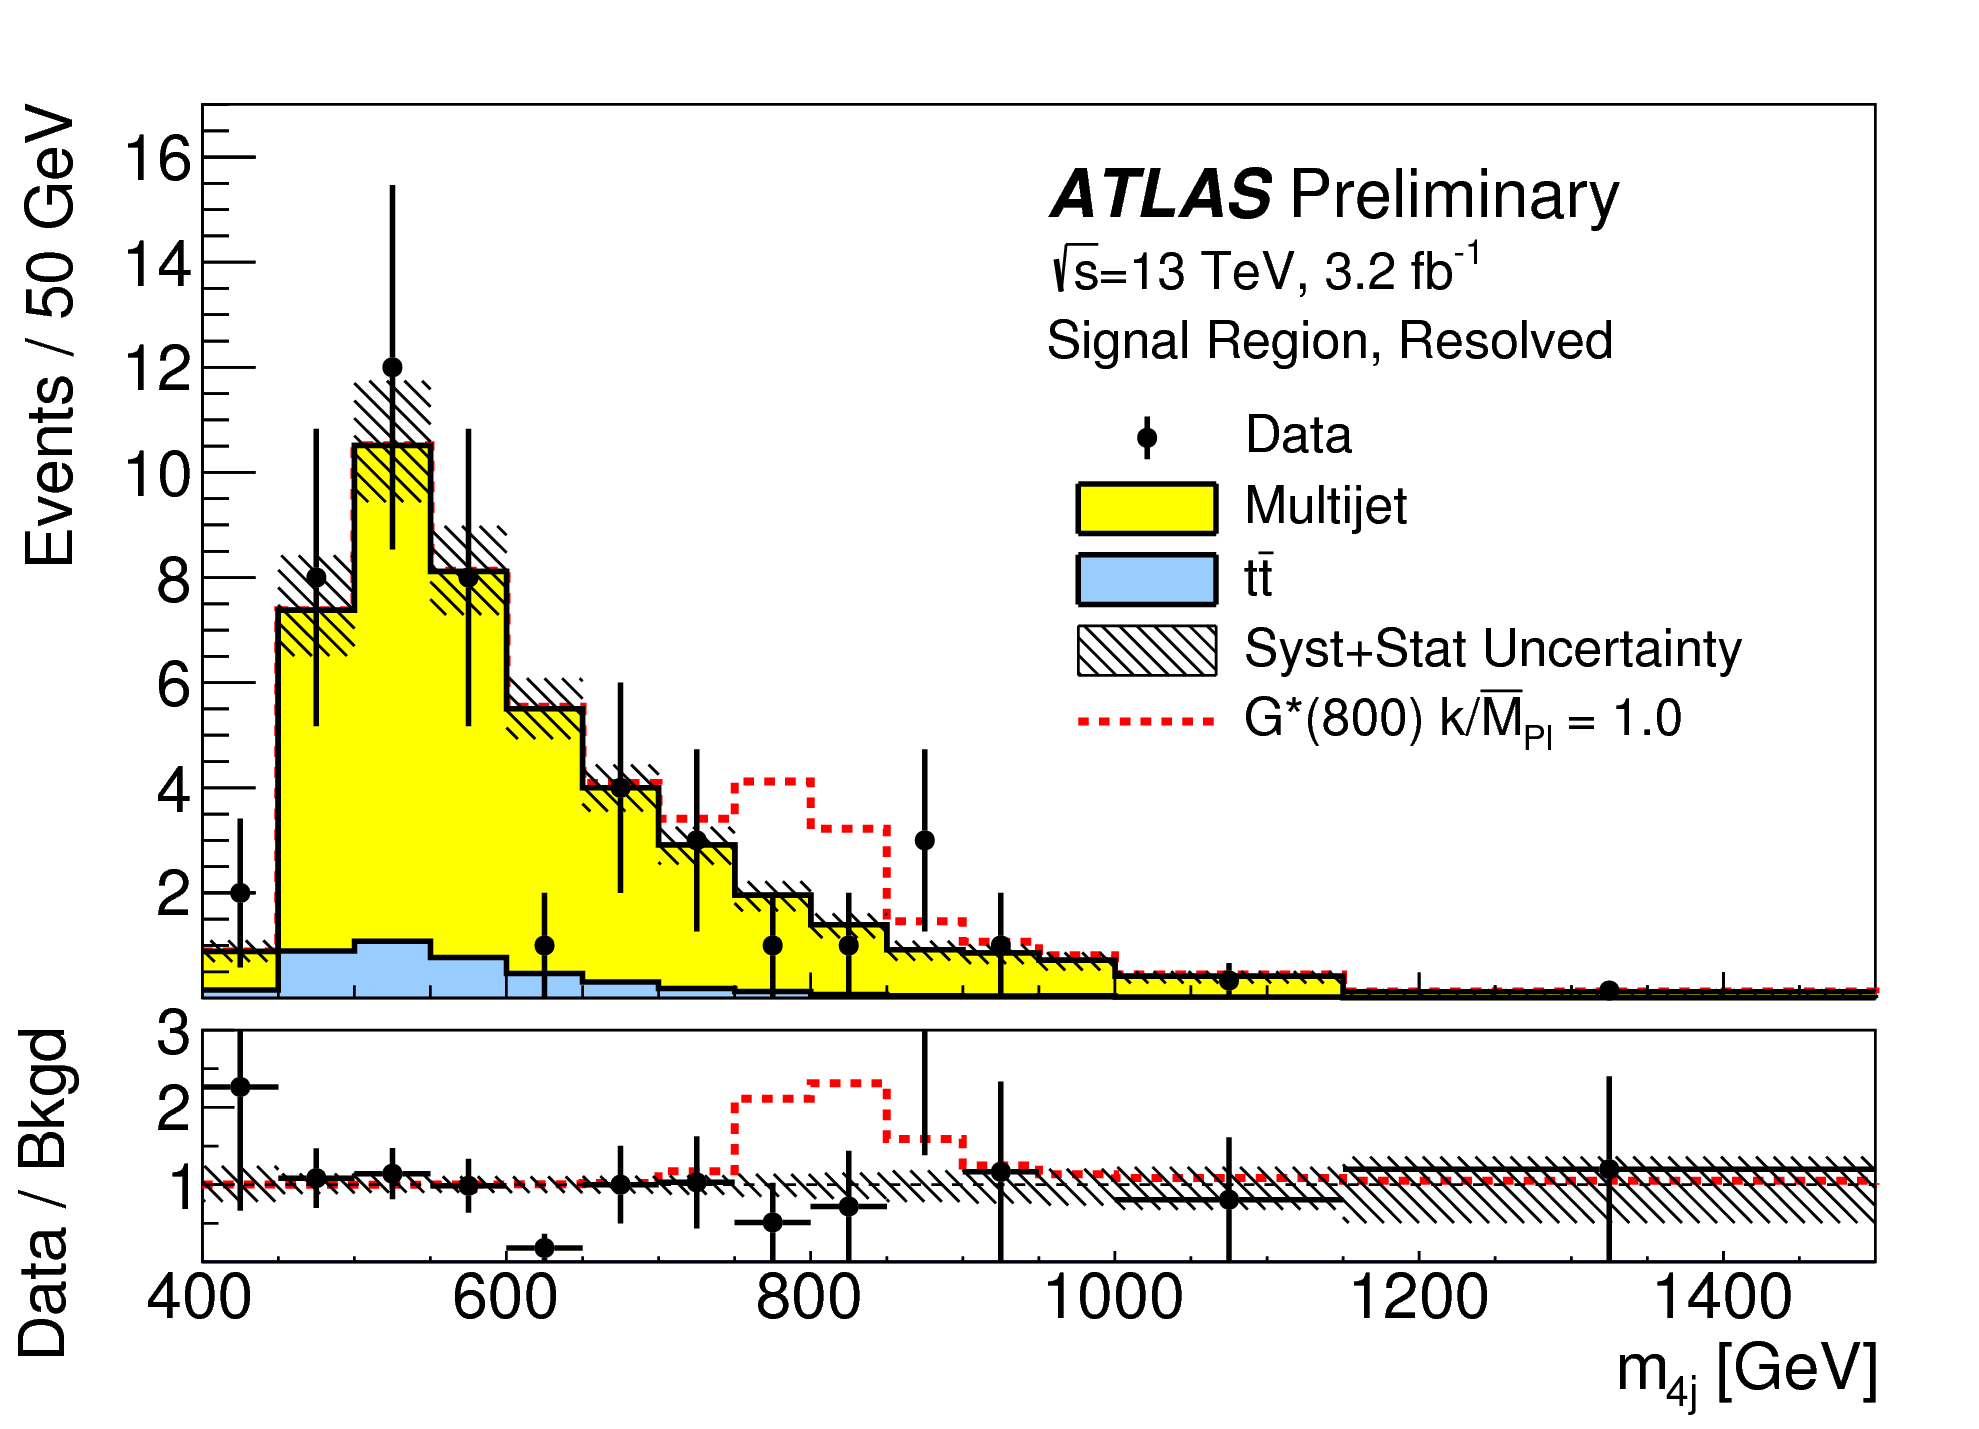
\includegraphics[width=0.6\textwidth]{figures/Resolved_signal}


   \caption{Di-jet invariant mass ($M_{2J}$) in the resolved signal region. Agraviton signal with $m_{\Gkk} = 800 \GeV$ and $c=1$ is overlaid. ~\cite{4bconf}.}
  \label{fig:ResolvedResults}
\end{figure}